\chapter{Introduction}
    The \gls{vrp} is one of the most extensively studied combinatorial problems. It is easy to define but hard to solve. The reason (\gls{vrp}) is attracting many researchers is the fact that finding a near-optimal solution in a reasonable time would have a great impact on many industries, especially in the domain of transportation and logistics. 
    
    The paradigm shift in logistics business models towards instant gratification of customers are pushing the planning systems to be flexible and dynamic. The environment is constantly changing and planning systems have to update its solutions in a short amount of time but maintain the best delivery efficiency.
    
    The problem objective of \gls{vrp} is simply finding the shortest route for multiple vehicles to serve all the given set of customers. The shortest route can be differently interpreted based on your minimalization criteria, e.g, traveled distance, time, or a combination of both. It was first proposed by Dantzig and Ramser \cite{truck-dispatching-problem} in 1959, and since then researchers are coming up with different approaches how to solve the problem. 

    In the real world, the general VRP problem is not enough to solve the business-related problems. \gls{vrp} has multiple variants adding various constraints such as capacity, demand or time windows for given set of customers. The \gls{vrptw} is main focus of this thesis and we will be looking at some novel approaches how to solve it with \gls{ai}.
    
    Solving any kind of variation of \gls{vrp} via \gls{ai} results in instant geneated solution. Solving any kind of variation of \gls{vrp} via \gls{ai} results in instant geneated solution. Solving any kind of variation of \gls{vrp} via \gls{ai} results in instant geneated solution. Solving any kind of variation of \gls{vrp} via \gls{ai} results in instant geneated solution.
    
    \begin{figure}[ht]
        \centering
        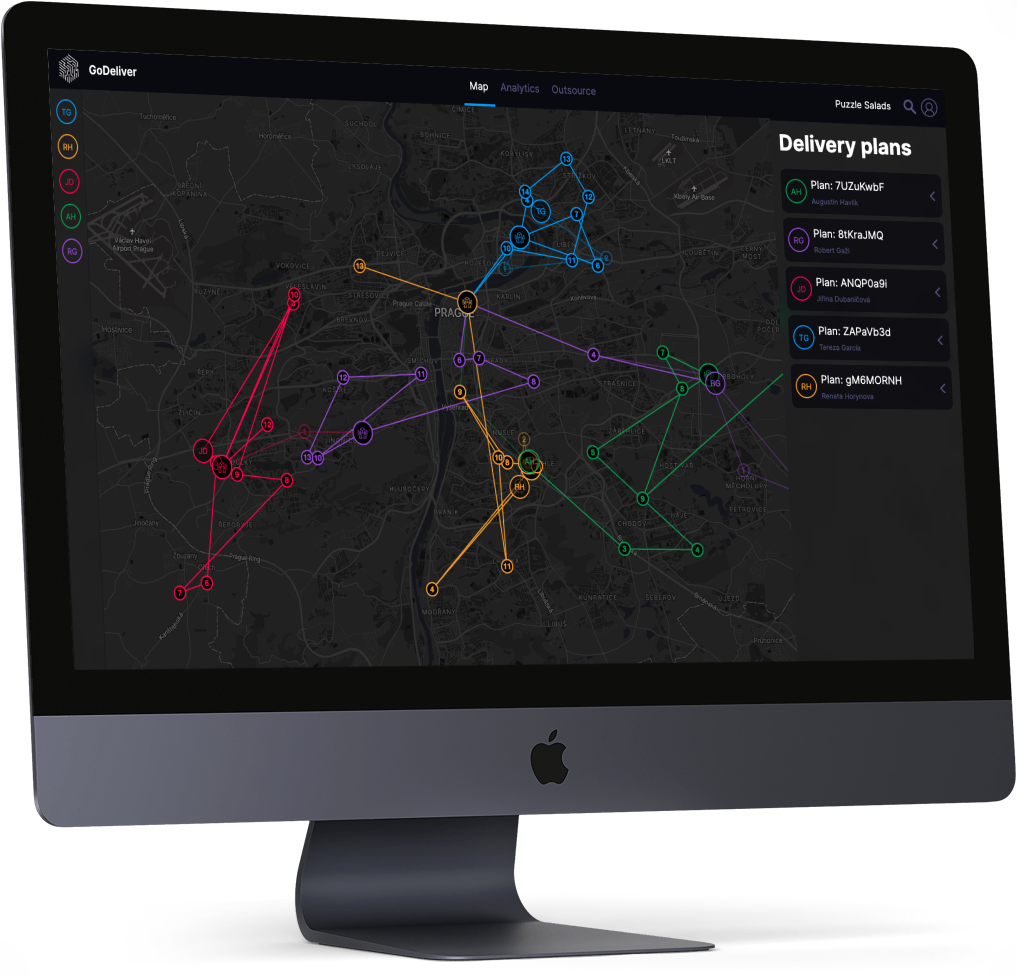
\includegraphics[width=0.75\textwidth]{resources/intro/godeliver-dashboard.png}
        \caption{GoDeliver dashboard illustrating the vehicle routing problem with time windows}
        \label{fig:godeliver_dashboard}
    \end{figure}

\section{Vehicle Routing Problem Definition}
    
    The general \gls{vrp} can be defined as a problem in a complete graph $G=(V,E)$ of finding the optimal permutation $\pi_l = (\pi_0, \cdots, \pi_m)$ of nodes $V$ all starting from a node $v_0$ for given number of paths $k$ which results in minimal traversal cost where $\forall v \in (V \setminus v_0)$ are visited only once. \gls{vrp} is generalization of \gls{tsp} which only has one path.
    
    \begin{figure}[ht]
        \centering
        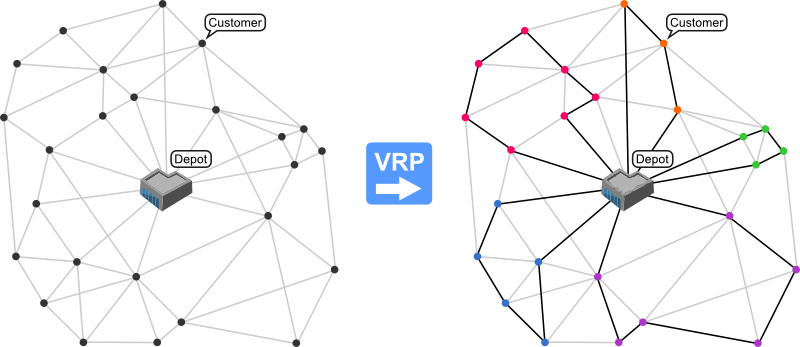
\includegraphics[width=0.75\textwidth]{resources/intro/vrp-graph.png}
        \caption{Intuitive view of \gls{vrp} instance on left and proposed solution for 5 vehicles on the right \cite{vrp-malaga}}
        \label{fig:vrp-graph}
    \end{figure}
    
    Let's introduce our used notation and its real-world interpretation.
    \begin{itemize}
        \item $G=(V,E)$ is a complete undirected graph
        \begin{itemize}
            \item Network of routes
        \end{itemize}
        \item $v_0$ is the initial node
        \begin{itemize}
            \item A depot
        \end{itemize}
        \item $V_1 = (v_1, \cdots, v_n)$ nodes expect the initial node
        \begin{itemize}
            \item Geographically scattered location of customers
        \end{itemize}
        \item $E = \{(v_i, v_j)| v_i, v_j \in V, i \neq j\}$ with associated weight as a cost $c: E \to \mathbb{N}^+$
        \begin{itemize}
            \item A single route between two locations with associated cost, e.g., distance.
        \end{itemize}
        \item $R_i \subset V$ is a path but starts and ends at $v_0$
        \begin{itemize}
            \item Route visit a subset of customers starting and ending at a depot, it can be referred to it as a delivery plan.
        \end{itemize}
        \item $k$ number of paths
        \begin{itemize}
            \item Number of vehicles
        \end{itemize}
        \item $R = R_1, \cdots, R_k$ is a set of paths
        \begin{itemize}
            \item All routes (delivery plans) for a given instance of \gls{vrp}.
        \end{itemize}
        \item $\pi = (\pi_1, \cdots, \pi_k)$ solution for a given instance of \gls{vrp}.
        \begin{itemize}
            \item Customer locations in visiting order for multiple vehicles.
        \end{itemize}
    \end{itemize}
    
    Solution for \gls{vrp} of routes $R_k$ is feasible only if each node $V_1$ is visited once.
    
    The cost of route $R_i$ which we aim to minimize is the sum of its weights (costs). If we operate in Euclidean space, then it is L2 norm of route locations.
    \begin{equation}
        C(R_i) := \sum_{i \in R} d_i \leq Q TODO
    \end{equation}
    
    The cost of \gls{vrp} solution is a sum of route costs.
    \begin{equation}
        C(R) := \sum_{i \in R} d_i \leq Q TODO
    \end{equation}
    
\section{Vehicle Routing Flavors}
Our modern world heavily relies on complex logistics networks to ship your goods from one side of the world to your doorstep. In order to synchronize This takes a multi-modal planning be planned and that is the reason why other flavours and varients of \gls{vrp} has been studied and implemented in real world usecases.

    \begin{figure}[ht]
        \centering
        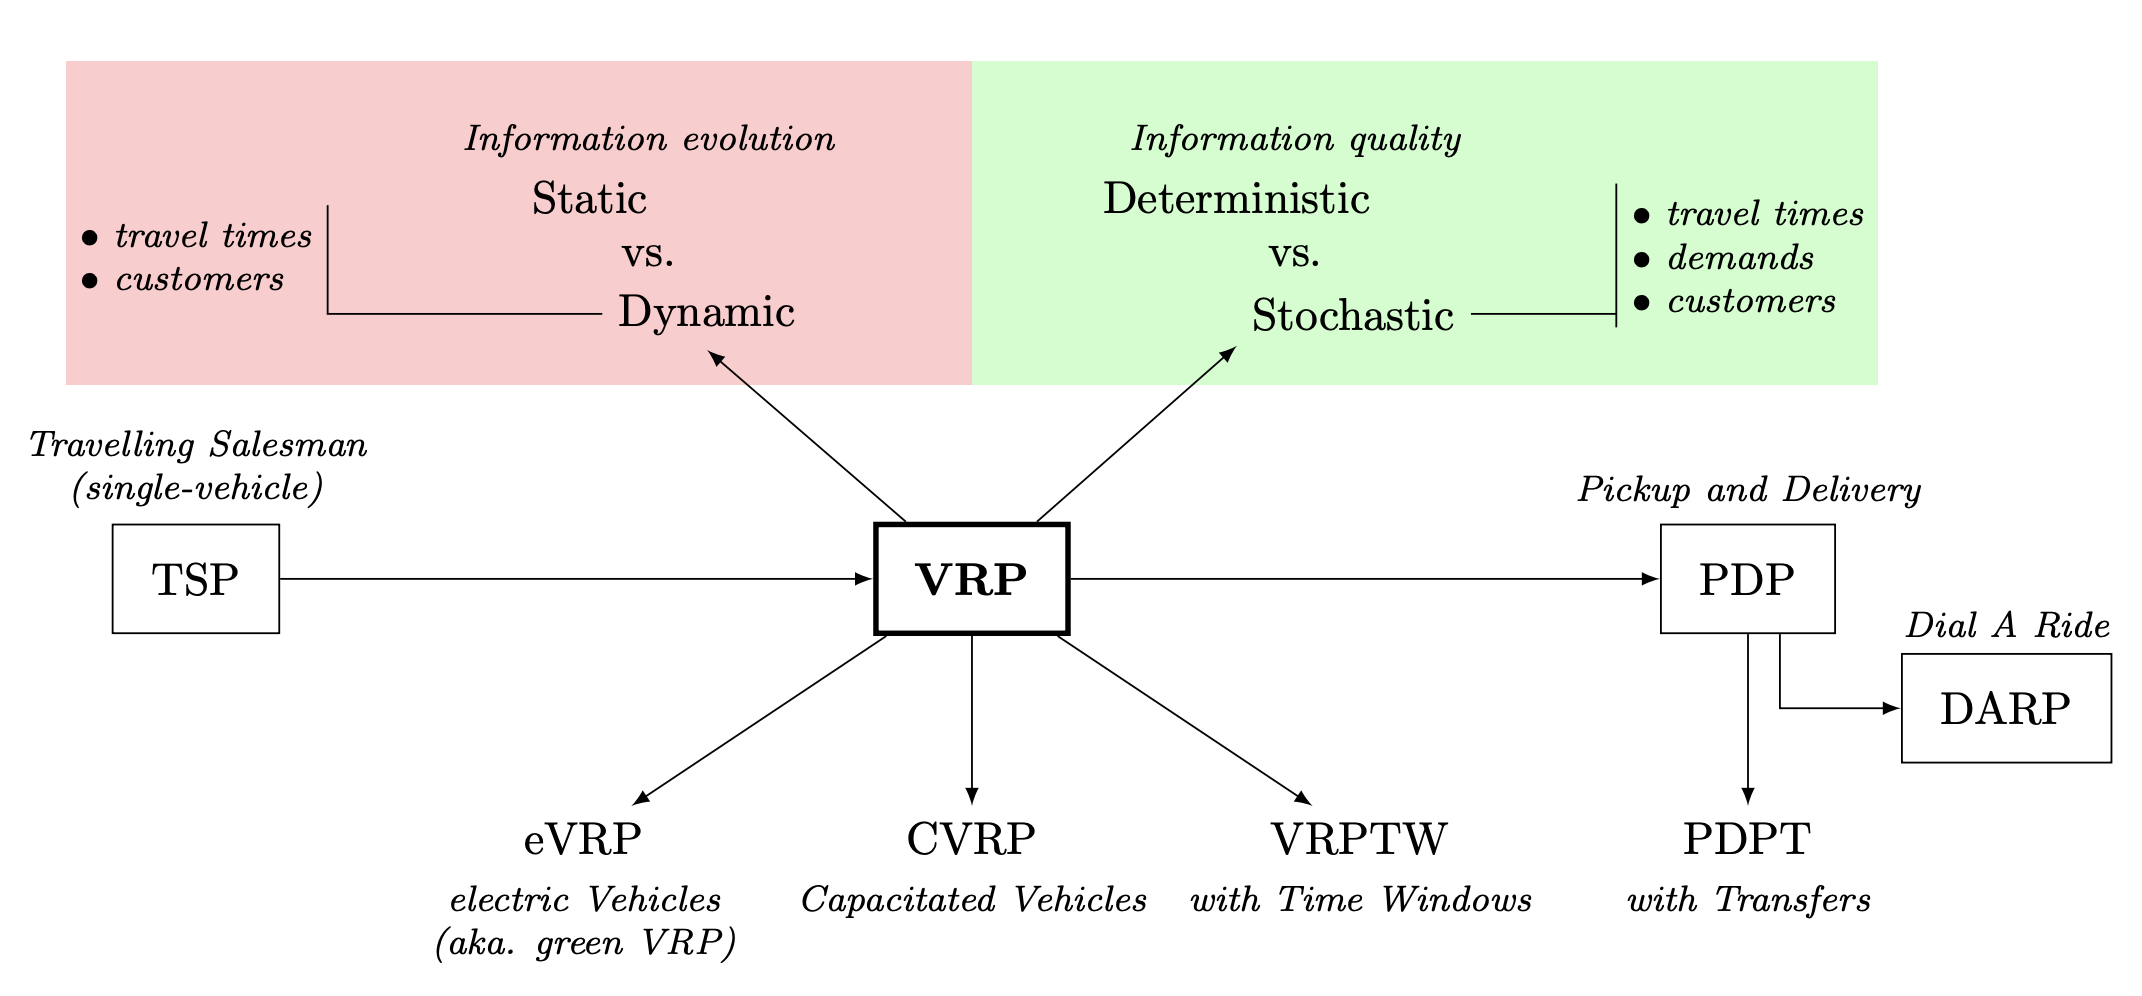
\includegraphics[width=1.0\textwidth]{resources/intro/vrp-flavours.png}
        \caption{Taxonomy of VRPs \cite{bono-stochastic-vrp}}
        \label{fig:vrp-flavours}
    \end{figure}

The sections bellow will be desctibing each flavours of shown in \ref{fig:vrp-flavours}

    \subsection{Capacited Vehicle Routing Problem}
    The \gls{cvrp} extends the regular \gls{cvrp} in introducing a capacity element for each customer. In the literature, it is sometimes referred to as a demand. The customer's demand is $d \in \mathbb{N}^+$ which may represent capacity in the form of weight, size but also in some abstract concepts such as a basket of apples. Additionally, each vehicle has a predefined capacity $Q > 0$.
    
    The \gls{cvrp} extends the solution feasibility formula by the following capacity constrain.
    \begin{equation}
        q(R) := \sum_{i \in R} d_i \leq Q
    \end{equation}
    
    If the vehicle capacity of the fleet stays the same, we are dealing with \gls{cvrp} with homogenous fleet. A fleet with varying capacity for each vehicle is a heterogenous fleet.
    
    \subsection{Vehicle Routing Problem with Time Windows}
    The \gls{vrptw} extends the regular \gls{vrp} by time constraint for each customer. Customers have assigned time window interval $[e_i, l_i]$ where $e_li < l_i$, is the request when a vehicle is supposed to visit the node. The time window can be either implemented as a hard constraint
    
    We consider time windows as a soft constraint, every time window can be violated barring a penalty cost. 
    
    In this thesis, we will be focusing on soft contrains for time windows because the lead to 
    
    Fesability - soft constraint
    
    \subsection{Pick and Deliver}
    TODO
    \subsection{Static Vehicle Routing Problem}
    TODO
    \subsection{Dynamic Vehicle Routing Problem}
    TODO
    \subsection{Deterministics Vehicle Routing Problem}
    TODO
    \subsection{Stochastic Vehicle Routing Problem}
    TODO
    
\section{Real-world Applications}
 Since then, a large part of the OR community has been devoted
to this problem which naturally arises in a large variety of practical applications. This
trend has been reinforced by the explosion of consumer direct delivery in the beginning of
the century. As an example of this explosion, UPS ground delivered around 11.5 million
packages in 19931
, against around 5.5 billion packages in 20192
.

Vehicle routing problems, among the most studied in combinatorial optimization, arise in many practical contexts (freight distribution and collection, transportation, garbage collection, newspaper delivery, etc.). Operations researchers have made significant developments in the algorithms for their solution, and Vehicle Routing: Problems, Methods, and Applications, Second Edition reflects these advances. The text of the new edition is either completely new or significantly revised and provides extensive and complete state-of-the-art coverage of vehicle routing by those who have done most of the innovative research in the area; it emphasizes methodology related to specific classes of vehicle routing problems and, since vehicle routing is used as a benchmark for all new solution techniques, contains a complete overview of current solutions to combinatorial optimization problems. It also includes several chapters on important and emerging applications, such as disaster relief and green vehicle routing. Audience: This book is intended for both researchers and graduate level students in operations research and applied mathematics. Practitioners will find this book particularly useful. Readers need a basic knowledge of the main methods for the solution of combinatorial optimization problems.